\chapter{Applied Case Study: Commercial Storyboard Analysis}
\label{ch:concept-to-sequence}
\index{storyboards!from concept}
\index{commercial production}

\begin{chapterabstract}
This chapter applies theoretical frameworks from previous chapters to real-world commercial production through detailed case study analysis. Using a Logitech G502 X PLUS esports mouse advertisement as the primary example, we demonstrate the complete workflow from concept development to finished 8-second commercial sequence. The chapter deconstructs style directives—the visual masterplans that establish tonality, color palettes, rhythm types, and camera movement logic. We examine shot-by-shot Prompt construction, analyzing how each text segment corresponds to specific camera parameters, lighting conditions, and motion dynamics. The case study reveals the relationship between linguistic precision and visual output quality, demonstrating how AI functions as cinematographer executing directorial commands. Additional commercial applications explored include brand storytelling, product launches, social media campaigns, and corporate communications. Technical considerations address format specifications, platform optimization, and client delivery requirements. Through this applied analysis, readers bridge the gap between theoretical understanding and professional practice, gaining confidence to execute commercial AI video projects. The chapter establishes practical templates and workflows transferable to diverse commercial contexts.
\end{chapterabstract}

In previous chapters, we learned how to construct an impressive single-shot scene, but in cinematic narrative, one shot—however perfect—is merely ``one note'' in visual storytelling. What truly grants a work emotional tension and rhythmic beauty is \textbf{the connection, transition, and breathing between shots}\index{shot connections}—a dynamic flow that gives imagery rhythm, beat, progression, and breath.

In AI-driven video creation, especially when using text-generation systems like \textbf{Sora 2}\index{Sora 2}, the storyboard is no longer hand-drawn static sketches but a form of \textbf{directorial art of controlling shots through language}\index{language as directorial tool}. Each Prompt you write isn't merely describing imagery but constructing the rhythm of time and space. Writing ``shot language''\index{shot language} has become the core skill of AI directors.

\section{From Shot to Sequence: The Logic of AI Directors}
\label{sec:ai-director-logic}
\index{AI director!logic}

Traditional directors use ``shot language'' to express characters and emotions when conceptualizing shots; in AI video creation, this language transforms into the structure and sequence of text. Each line of Prompt actually corresponds to a shot segment, a set of camera parameters, a kind of light and motion rhythm control.

AI's strength doesn't lie in understanding abstract stories but in ``executing commands.''\index{AI!command execution} Therefore, you need to use extremely precise syntax to tell it: where the frame begins, when it advances, how it ends.

In other words—\textbf{AI is the cinematographer; you are the director}\index{AI as cinematographer}. You don't need to hold the camera, but you must write shot language. The precision and rhythmic sense of Prompts determine the ``directorial prowess'' of generated video.

\section{Commercial Storyboard Case Study: Logitech G502 X PLUS}
\label{sec:logitech-case}
\index{case study!Logitech}
\index{product advertising}

To make this concept more intuitive, we'll use ``\textbf{Logitech G502 X PLUS}—an 8-second esports mouse advertisement'' as an example. The goal is to help beginners understand: why time should be divided this way, language written this way, rhythm laid out this way.

\begin{figure}[H]
\centering
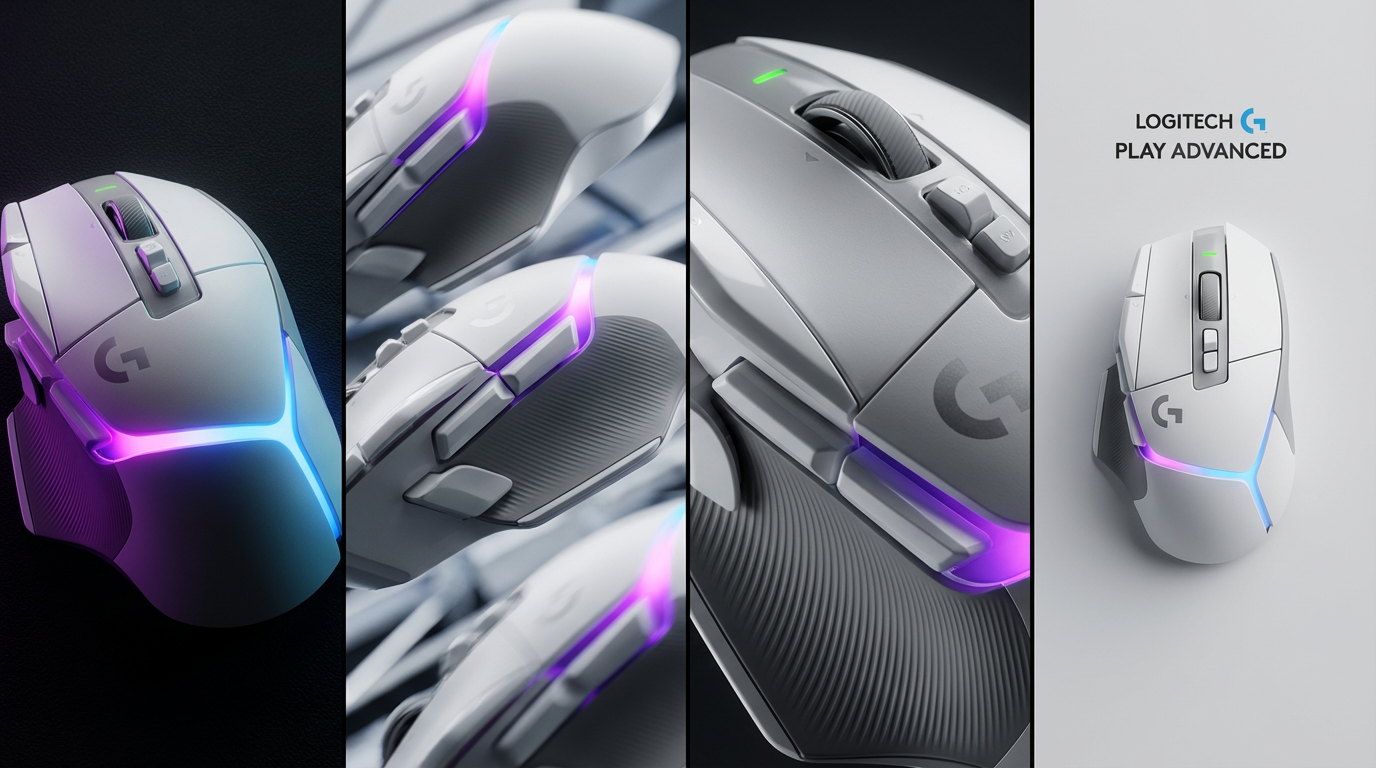
\includegraphics[height=\figheight]{Fig8-1.png}
\caption{Logitech G502 X PLUS—8-second esports product showcase structure \\ \authorcreated}
\label{fig:logitech-structure}
\index{figure!product advertising}
\end{figure}

\subsection{Overall Style Directive}
\label{subsec:style-directive}
\index{style directive}

An 8-second ultra-high-definition, futuristic esports technology commercial. Employs high-contrast lighting, dynamic cinematography, and fast cuts, with primary color palette of deep blue and luminous LIGHTSYNC RGB, emphasizing speed, precision, and wireless freedom.

This ``style directive''\index{style directive} is the \textbf{visual masterplan}\index{visual masterplan} of the entire project. In traditional film production, it's equivalent to the ``visual alignment meeting'' between director and cinematographer—where you establish the film's tonality, primary hues, rhythm type, and camera movement logic. When AI models generate based on this, they'll transform these keywords into color matrices, contrast control, motion blur parameters, and other internal visual features.

\begin{table}[H]
\centering
\caption{Style directive components and purposes \\ \authorillustration}
\label{tab:style-components}
\index{table!style directives}
\small
\begin{tabular}{p{3cm}p{5cm}p{6cm}}
\hline
\textbf{Function} & \textbf{Phrasing} & \textbf{Purpose} \\
\hline
Work positioning & ``An 8-second ultra-HD commercial'' & Define video length and type, control rhythm scope \\
Thematic direction & ``Futuristic esports tech'' & Let model understand style is cold, electronic, futuristic \\
Visual style & ``High contrast, fast cuts, dynamic shots'' & Control editing speed and light conflict sense \\
Color syntax & ``Deep blue + LIGHTSYNC RGB'' & Lock neon cool palette, ensure visual consistency \\
\hline
\end{tabular}
\end{table}

These four elements constitute a human director's ``scheduling sheet''\index{scheduling}: they specify photographic baseline, color relationships, lighting style, and rhythm density. Without this layer of definition, AI-generated imagery often suffers from style drift and rhythm disorder.

\section{Why Write a ``Scene Timeline''}
\label{sec:scene-timeline}
\index{scene timeline}
\index{temporal structure}

Many beginners are accustomed to writing ``showcase product, feature LOGO, demonstrate function'' without temporal sequence. AI models won't independently understand ``introduction-development-turn-conclusion''; they need human-established ``temporal segmentation''\index{temporal segmentation}—this is the significance of a ``scene timeline.''

For example:

\begin{Prompt}
0--1.5 sec: Visual ignition point, lights activate.

1.5--4.5 sec: Core showcase, rhythm ascends.

4.5--6.0 sec: Texture intensification, slow-motion transition.

6.0--8.0 sec: Thematic resolution, brand freeze.
\end{Prompt}

When Sora 2 reads this structure, it automatically divides video into four shot blocks. Each block corresponds internally to independent motion parameters and exposure logic. In other words, the timeline is the secret to making AI ``breathe.''\index{AI breathing}

In traditional advertising, this rhythmic structure is called ``audiovisual curve''\index{audiovisual curve}: Rise → Peak → Relax → Closure. When analyzing Prompts, AI models also generate video with similar psychological rhythm. Recent research has demonstrated that movie editing significantly influences spectators' time perception, with edited sequences being perceived as longer than unedited ones \citep{kovarski2022movie}. Write clearly, and video flows naturally.

\section{The Interactive Mechanism of Shots and Language}
\label{sec:shots-language-interaction}
\index{shot-language interaction}

\subsection{0--1.5 sec: The Close-up Launch}
\label{subsec:closeup-launch}
\index{close-up launch}

\textbf{Keywords:} Macro Shot, dark field illuminating, RGB flow, electronic pulse.

Starting from extreme close-up is a classic strategy for capturing attention. When AI reads ``Macro Shot,'' it automatically invokes shallow depth-of-field models, intensifying product texture; ``dark field illuminating'' triggers light gradient logic; ``electronic pulse'' drives imagery to exhibit slight oscillation and light flow flicker. All this isn't random but textually-triggered \textbf{visual algorithmic response}\index{algorithmic response}.

\textbf{Voiceover:} ``Light speed, instant awakening.''

Short sentence, strong rhythm, aligned with sound effects. Although AI currently doesn't generate actual sound, it simulates audio-visual synchronization rhythm sense through shot movement acceleration and light frequency. This synesthetic visual effect\index{synesthetic visual effect} carries tremendous impact in advertising.

\subsection{1.5--4.5 sec: High-Speed Control}
\label{subsec:highspeed-control}
\index{high-speed control}

This is the rhythm's main peak.

\textbf{POV (first-person perspective)}\index{POV shot} makes viewers ``become the player,'' while ``side close-up'' creates dynamic variation during switching. Keywords ``no delay'' ``lightweight'' trigger AI's internal speed parameters, causing imagery background to exhibit high-frequency blur (Motion Blur)\index{motion blur}.

\textbf{Voiceover:} ``Wireless freedom, feel LIGHTFORCE's crispness.''

When analyzing semantics, AI identifies ``contrast structure'' (Freedom vs. Precision) and automatically arranges symmetrical shots in the middle section—one showcasing action freedom, one showcasing mechanical detail. This is the logic of language-driven visuals.

\subsection{4.5--6.0 sec: The Detail Power}
\label{subsec:detail-power}
\index{detail power}

Rhythm deceleration is key to advanced sophistication.

``Slow motion + RGB light burst'' makes AI adjust frame rate and lighting parameters, simulating precision mechanical feedback. The setup of three clicking sounds, though silent, Prompts the model to generate three light flash rhythms—this is so-called ``phantom audio sync'' (implied sound synchronization).\index{phantom audio sync}

This segment provides emotional breathing space for the audience, transitioning from high-speed stimulation to stable trust, laying psychological groundwork for brand credibility.

\subsection{6.0--8.0 sec: Final Statement}
\label{subsec:final-statement}
\index{final statement}

Imagery stabilizes, camera pulls back, LOGO centers. Color tone shifts from blue to black; soundtrack (i.e., rhythm) gradually stops.

Voiceover ``Victory, from now controlled by you'' forms opening-closing symmetry, echoing the opening sentence ``Light speed awakening.'' After AI identifies this structure, it automatically intensifies the closing brand statement effect, generating gradual-dark, focus, freeze closing shots.

\textbf{Summary Rhythm Line:}

\begin{Prompt}
Launch → Accelerate → Solidify → Freeze.
\end{Prompt}

\section{The Collaborative Principle of Sound and Image}
\label{sec:sound-image-collaboration}
\index{sound-image collaboration}

AI's ``understanding'' of sound isn't generating sound waves but translating sound Prompts into visual rhythm. The following table illustrates its response mechanism:

\begin{table}[H]
\centering
\caption{Sound effects and AI visual responses \\ \authorillustration}
\label{tab:sound-visual}
\index{table!sound-visual mapping}
\begin{tabular}{ll}
\hline
\textbf{Sound Effect Description} & \textbf{AI Visual Response} \\
\hline
Bass vibration & Camera produces slight shake, lights flicker \\
Soundtrack accelerates & Cutting frequency rises, motion blur increases \\
Soundtrack gradually stops & Camera stabilizes, light and shadow soften \\
Clicking sound & Light brightens or mechanical action coordinates with beat \\
\hline
\end{tabular}
\end{table}

Therefore, sound effect descriptions in text are actually \textbf{invisible commands for shot rhythm}\index{invisible rhythm commands}, enabling static imagery to ``hear the beat.''

\section{The Golden Temporal Structure of 8 Seconds}
\label{sec:eight-second-structure}
\index{eight-second structure}
\index{golden duration}

In the advertising production industry, commonly used short film lengths are 6 seconds, 8 seconds, and 15 seconds. Among these, \textbf{8 seconds}\index{8-second format} is the duration with the greatest visual memory effect—sufficient to showcase a brand concept yet not so long as to cause attention decline.

Sora 2's internal rendering logic is based on 24fps frame rate; an 8-second video comprises approximately 192 frames. The AI model maps your temporal commands onto frame intervals, with each time segment automatically generating independent shot groups. Such video won't transition abruptly nor extend randomly.

\section{Replicable Template: The Power of Structure}
\label{sec:replicable-template}
\index{templates!commercial}

\begin{verbatim}
[Overall Style Directive]
An 8-second ultra-high-definition (4K/8K) commercial short film,
employing high-contrast lighting, dynamic cinematography, and fast editing.
Primary color palette: [Insert Color]. Emphasizing product characteristics: [Insert Features].

[Scene Timeline]
0-1.5 sec: Launch shot (close-up + lights activate)
1.5-4.5 sec: Core feature showcase (high-speed + contrast)
4.5-6.0 sec: Detail expression (slow-motion + feedback)
6.0-8.0 sec: Thematic resolution (static + LOGO + slogan)

[Sound Effects/Voiceover]
—— Each segment one short sentence, controlled within 4~7 words.
\end{verbatim}

This structure can seamlessly migrate to any product type—from tech hardware to beauty skincare, from automotive ads to smart appliances. As long as rhythm proportions remain consistent, Sora 2 will automatically understand your narrative beat.

\section{AI is a Cinematographer, Not a Magician}
\label{sec:ai-cinematographer}
\index{AI!limitations}
\index{directorial precision}

Common misconceptions suggest AI can ``create masterpieces from single sentences,'' but professional directors understand: \textbf{Shot division requires systematic rhythm construction, not spontaneous inspiration}\index{systematic rhythm}.

Detailed Prompts enable AI to function as a precise production team; vague Prompts result in aesthetically pleasing but logically inconsistent output.

Effective AI storyboard writing requires:

\begin{Prompt}
Directorial precision in language produces cinematic results in AI.
\end{Prompt}

AI functions as an execution tool rather than creative replacement; it enables faster and more precise implementation of directorial vision. Users must develop skills in controlling lighting, composition, rhythm, and movement through textual description, transforming Prompts into \textbf{language-based production scripts}.\index{language-based scripts}

Professional AI direction depends on systematic Prompt construction rather than command quantity.

\section*{Practical Exercises}
\index{practical exercises}

\begin{quote}
\textit{\textbf{Timeless Principle:} Even as interfaces evolve and platforms update, the underlying visual logic---light, composition, rhythm, and emotional resonance---remains eternal. Master these fundamentals, and you will adapt effortlessly to any future tool.}
\end{quote}

\textbf{Exercise 1: 8-Second Commercial Creation}
\begin{enumerate}
\item Choose a product from your daily life (smartphone, coffee mug, book, etc.)
\item Create a 4-segment commercial following the Logitech template:
   \begin{itemize}
   \item Segment 1 (0-1.5s): Product launch/reveal
   \item Segment 2 (1.5-4.5s): Feature showcase
   \item Segment 3 (4.5-6.5s): Detail highlight
   \item Segment 4 (6.5-8s): Brand closing
   \end{itemize}
\item Write detailed Prompts for each segment, including camera movements, lighting, and timing
\item Generate the video and analyze rhythm effectiveness
\end{enumerate}

\textbf{Exercise 2: Competitive Analysis Practice}
\begin{enumerate}
\item Select 3 successful commercials from different brands in the same industry
\item Break down each commercial into 1.5-second segments
\item Identify the narrative structure and timing patterns
\item Recreate one commercial using AI with your own product
\item Compare the emotional impact and engagement effectiveness
\end{enumerate}

\textbf{Exercise 3: Multi-Platform Adaptation}
\begin{enumerate}
\item Create a master 8-second commercial for a product
\item Adapt it for different platforms:
   \begin{itemize}
   \item TikTok version (vertical format, trending audio)
   \item Instagram Reels (square format, hashtag integration)
   \item YouTube Shorts (horizontal format, longer attention span)
   \end{itemize}
\item Test each version's performance and engagement
\end{enumerate}

\section*{Commercial Production Checklist}
\index{commercial checklist}

\subsection*{Pre-Production Checklist}
\begin{itemize}
\item[$\square$] Product research and competitive analysis completed
\item[$\square$] Target audience and platform requirements defined
\item[$\square$] 8-second structure planned with precise timing
\item[$\square$] Key message and call-to-action identified
\item[$\square$] Visual style and brand guidelines established
\end{itemize}

\subsection*{Production Checklist}
\begin{itemize}
\item[$\square$] Each segment Prompt includes specific timing (0-1.5s, etc.)
\item[$\square$] Camera movements and angles specified
\item[$\square$] Lighting conditions and mood described
\item[$\square$] Product positioning and visibility optimized
\item[$\square$] Brand elements and colors incorporated
\item[$\square$] Audio cues and voiceover timing planned
\end{itemize}

\subsection*{Post-Production Checklist}
\begin{itemize}
\item[$\square$] Rhythm and pacing match 8-second golden rule
\item[$\square$] Visual transitions are smooth and purposeful
\item[$\square$] Audio levels consistent (-14 LUFS standard)
\item[$\square$] Brand message clear and memorable
\item[$\square$] Call-to-action prominent and actionable
\item[$\square$] Platform-specific requirements met (aspect ratio, duration)
\end{itemize}

\section*{Prompt Templates}
\index{Prompt templates}

\subsection*{Template 1: Commercial Product Launch}
\begin{Prompt}
\textbf{[Product Entry]} + [Hero Shot] + [Feature Highlight] + [Lifestyle Context] + [Brand Closing]

Example: "Sleek smartphone emerges from darkness + rotating 360-degree hero shot + close-up of camera lens detail + person capturing sunset moment + logo appears with premium lighting"
\end{Prompt}

\subsection*{Template 2: 8-Second Commercial Structure}
\begin{Prompt}
\textbf{[0-1.5s Hook]} → [1.5-4.5s Showcase] → [4.5-7s Detail] → [7-8s Closing]

Example: "Quick montage of daily chaos → product solving the problem smoothly → close-up of key feature → satisfied user with brand logo"
\end{Prompt}

\subsection*{Template 3: Emotional Brand Storytelling}
\begin{Prompt}
\textbf{[Human Moment]} + [Product Integration] + [Emotional Payoff] + [Brand Connection]

Example: "Child's first bike ride + parent running alongside + moment of independence and joy + brand tagline about supporting life's moments"
\end{Prompt}

\section*{Chapter Summary}

Key actionable insights from commercial storyboard analysis:

\begin{itemize}
\item \textbf{8-Second Golden Rule}: Structure commercial content in 8-second segments for optimal platform performance and attention retention
\item \textbf{Template Replication}: Use the Logitech case structure (launch-showcase-detail-closing) as a universal commercial template
\item \textbf{Precise Timing}: Allocate specific time segments (0-1.5s, 1.5-4.5s, etc.) to maintain rhythm control
\item \textbf{Sound-Visual Coordination}: Limit voiceover to 4-7 words per segment to match visual pacing
\item \textbf{Directorial Precision}: Write detailed Prompts like a cinematographer's script rather than vague creative briefs
\end{itemize}
